
\subsection{Op basis van verstoring door aggregatie}

\subsubsection{Aanpak door het gedistribueerd aggregeren van offline profielen door Shokri et al. \cite{LCA-CONF-2009-014}}

In tegenstelling tot de oplossing met randomisatie worden in deze methode niet de aparte ratings verstoord maar eerder de volledige profielen. De service provider berekent dan aanbevelingen op basis van deze verstoorde profielen. 

Een gebruiker heeft drie verschillende profielen. Het eerste profiel wordt bijgehouden aan de kant van de gebruiker en is enkel opgesteld met ratings geleverd door de gebruiker zelf. Dit profiel wordt nooit opgevraagd door de service provider. Een tweede profiel, het offline profiel genoemd, is een kopie van het eerste profiel uitgebreid met ratings uit offline profielen van andere gebruikers. Het online profiel dat bijgehouden wordt aan de kant van de server is eigenlijk een kopie van het offline profiel en haalt periodiek updates op van de client. Op basis van dit profiel zal de server zijn aanbevelingen berekenen.

Men kan gebruikers en items voorstellen als nodes in een graaf en ratings als verbindingen met gewicht tussen item en gebruiker. De client kan op een arbitraire manier contact met andere clients leggen. Bij een contact delen clients ratings van hun offline profielen. Hierbij kan de client vanzelfsprekend zijn eigen ratings behouden. Omdat deze interactie enkel tussen clients gebeurt heeft de server geen weet van welke clients onderling ratings delen. Hij weet dus ook niet welke ratings van het offline profiel van de gebruiker zelf  zijn en welke van een andere client afkomstig zijn.  Aangezien de clients onderling enkel gegevens van hun offline profiel delen geldt hetzelfde tussen gebruikers en is er dus ook een graad van user-user privacy. Het kan dan ook gebeuren dat de server items aanbeveelt die de gebruiker al beoordeeld heeft. Het is aan de clientapplicatie zelf om hierin te schiften.

\begin{figure}[htpb]   
    \label{Figuur::aggregatiefig}      
  \begin{center}    
 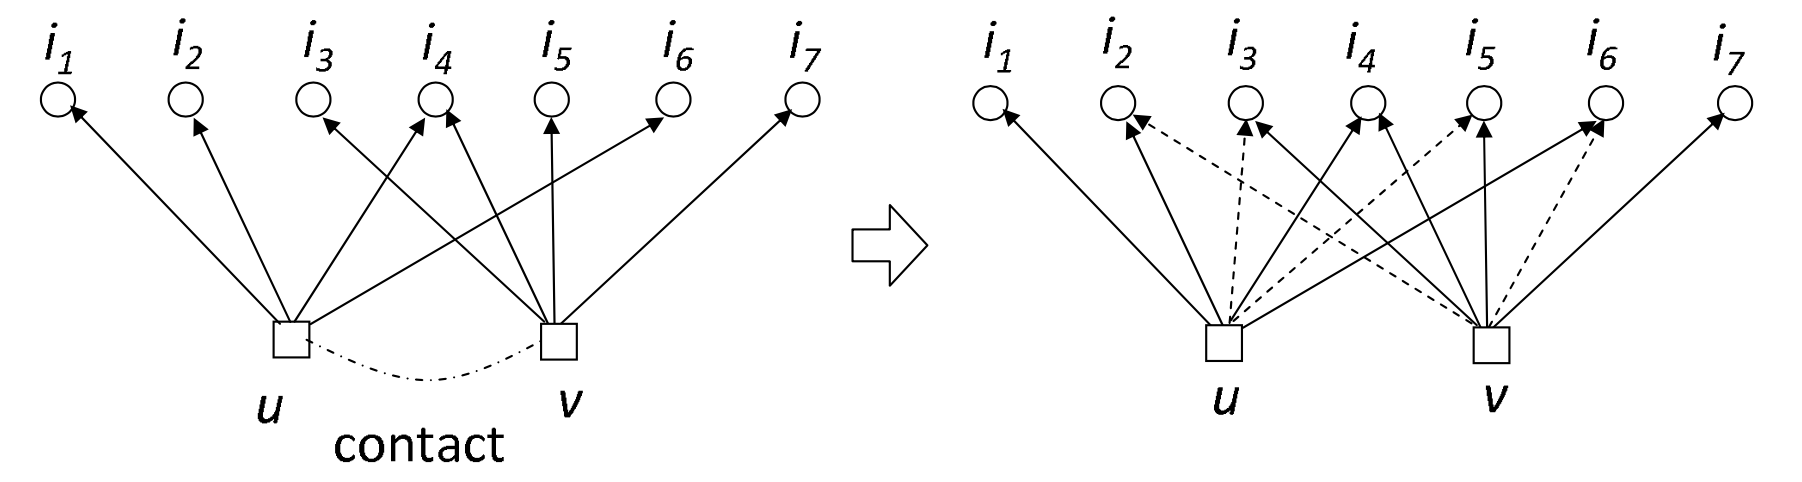
\includegraphics[scale=0.35]{fig/aggregatie}    
  \end{center}   
  \caption{Twee gebruikers wisselen ratings uit, uit \cite{LCA-CONF-2009-014}.}  
   \end{figure} 

Er moet vooraf bepaald worden welke ratings gedeeld worden tussen twee gebruikers en hoeveel. Shokri et al. geven hier verschillende opties voor. Alle ratings, een vast aantal ratings of het aantal ratings laten afhangen van de gelijkenis van twee gebruikers zijn mogelijkheden. De gelijkenis tussen twee gebruikers wordt privacyvriendelijk berekend met een methode van Lathia et al. \cite{lath}. Welke ratings worden gebruikt kan willekeurig gekozen worden of er kan een voorkeur gegeven worden aan de items die het minst geratet zijn over het hele systeem. Een onderzoek van Narayanan en Shmatikov \cite{nar} geeft aan dat een rating van een item, dat weinig beoordeeld is over alle users heen, sneller tot identificatie van een gebruiker kan leiden.  De optie om net deze ratings te delen tussen gebruikers heeft dus een positieve impact op de privacy.

De privacymaat wordt berekend op basis van de gelijkenis tussen de verstoorde online graaf en de originele graaf rekening houdende met aantal ratings per item. 
Als er gegevens met zes gebruikers per jaar uitgewisseld worden kan dit leiden naar een significante privacywinst van 0.68 de gebruiker naar de provider toe. bij een accuraatheidsverlies van 2\% . 


Belangrijke kenmerken :
\begin{itemize}
 
\item Deze methode is dan wel privacyvriendelijker dan de verstoring met randomisatie maar heeft toch zijn beperkingen.
\end{itemize}
Voordelen : 
\begin{itemize}
\item In tegenstelling tot de oplossing met randomisatie heeft hier de service provider geen idee welke items door de user zelf beoordeeld zijn. 
\item Weinig accuraatheidsverlies
\end{itemize}
Nadelen:
\begin{itemize}
\item Ratings van een offline profiel die lange tijd gelijk blijven hebben meer kans van die user zelf te zijn.
\item Het systeem krijgt de originele ratings van de gebruiker.

\end{itemize}
